
%% bare_jrnl.tex
%% V1.4b
%% 2015/08/26
%% by Michael Shell
%% see http://www.michaelshell.org/
%% for current contact information.
%%
%% This is a skeleton file demonstrating the use of IEEEtran.cls
%% (requires IEEEtran.cls version 1.8b or later) with an IEEE
%% journal paper.
%%
%% Support sites:
%% http://www.michaelshell.org/tex/ieeetran/
%% http://www.ctan.org/pkg/ieeetran
%% and
%% http://www.ieee.org/

%%*************************************************************************
%% Legal Notice:
%% This code is offered as-is without any warranty either expressed or
%% implied; without even the implied warranty of MERCHANTABILITY or
%% FITNESS FOR A PARTICULAR PURPOSE! 
%% User assumes all risk.
%% In no event shall the IEEE or any contributor to this code be liable for
%% any damages or losses, including, but not limited to, incidental,
%% consequential, or any other damages, resulting from the use or misuse
%% of any information contained here.
%%
%% All comments are the opinions of their respective authors and are not
%% necessarily endorsed by the IEEE.
%%
%% This work is distributed under the LaTeX Project Public License (LPPL)
%% ( http://www.latex-project.org/ ) version 1.3, and may be freely used,
%% distributed and modified. A copy of the LPPL, version 1.3, is included
%% in the base LaTeX documentation of all distributions of LaTeX released
%% 2003/12/01 or later.
%% Retain all contribution notices and credits.
%% ** Modified files should be clearly indicated as such, including  **
%% ** renaming them and changing author support contact information. **
%%*************************************************************************


% *** Authors should verify (and, if needed, correct) their LaTeX system  ***
% *** with the testflow diagnostic prior to trusting their LaTeX platform ***
% *** with production work. The IEEE's font choices and paper sizes can   ***
% *** trigger bugs that do not appear when using other class files.       ***                          ***
% The testflow support page is at:
% http://www.michaelshell.org/tex/testflow/



\documentclass[journal]{IEEEtran}
%
% If IEEEtran.cls has not been installed into the LaTeX system files,
% manually specify the path to it like:
% \documentclass[journal]{../sty/IEEEtran}

\usepackage[utf8]{inputenc} % Required for inputting international characters
\usepackage[flushleft]{threeparttable}
\usepackage{amsmath}
\usepackage{graphicx}
\usepackage{algorithm}
\usepackage[colorinlistoftodos]{todonotes}
\usepackage[colorlinks=true, allcolors=blue]{hyperref}
\usepackage[noend]{algorithmic}




% Some very useful LaTeX packages include:
% (uncomment the ones you want to load)


% *** MISC UTILITY PACKAGES ***
%
%\usepackage{ifpdf}
% Heiko Oberdiek's ifpdf.sty is very useful if you need conditional
% compilation based on whether the output is pdf or dvi.
% usage:
% \ifpdf
%   % pdf code
% \else
%   % dvi code
% \fi
% The latest version of ifpdf.sty can be obtained from:
% http://www.ctan.org/pkg/ifpdf
% Also, note that IEEEtran.cls V1.7 and later provides a builtin
% \ifCLASSINFOpdf conditional that works the same way.
% When switching from latex to pdflatex and vice-versa, the compiler may
% have to be run twice to clear warning/error messages.






% *** CITATION PACKAGES ***
%
%\usepackage{cite}
% cite.sty was written by Donald Arseneau
% V1.6 and later of IEEEtran pre-defines the format of the cite.sty package
% \cite{} output to follow that of the IEEE. Loading the cite package will
% result in citation numbers being automatically sorted and properly
% "compressed/ranged". e.g., [1], [9], [2], [7], [5], [6] without using
% cite.sty will become [1], [2], [5]--[7], [9] using cite.sty. cite.sty's
% \cite will automatically add leading space, if needed. Use cite.sty's
% noadjust option (cite.sty V3.8 and later) if you want to turn this off
% such as if a citation ever needs to be enclosed in parenthesis.
% cite.sty is already installed on most LaTeX systems. Be sure and use
% version 5.0 (2009-03-20) and later if using hyperref.sty.
% The latest version can be obtained at:
% http://www.ctan.org/pkg/cite
% The documentation is contained in the cite.sty file itself.






% *** GRAPHICS RELATED PACKAGES ***
%
\ifCLASSINFOpdf
  % \usepackage[pdftex]{graphicx}
  % declare the path(s) where your graphic files are
  % \graphicspath{{../pdf/}{../jpeg/}}
  % and their extensions so you won't have to specify these with
  % every instance of \includegraphics
  % \DeclareGraphicsExtensions{.pdf,.jpeg,.png}
\else
  % or other class option (dvipsone, dvipdf, if not using dvips). graphicx
  % will default to the driver specified in the system graphics.cfg if no
  % driver is specified.
  % \usepackage[dvips]{graphicx}
  % declare the path(s) where your graphic files are
  % \graphicspath{{../eps/}}
  % and their extensions so you won't have to specify these with
  % every instance of \includegraphics
  % \DeclareGraphicsExtensions{.eps}
\fi
% graphicx was written by David Carlisle and Sebastian Rahtz. It is
% required if you want graphics, photos, etc. graphicx.sty is already
% installed on most LaTeX systems. The latest version and documentation
% can be obtained at: 
% http://www.ctan.org/pkg/graphicx
% Another good source of documentation is "Using Imported Graphics in
% LaTeX2e" by Keith Reckdahl which can be found at:
% http://www.ctan.org/pkg/epslatex
%
% latex, and pdflatex in dvi mode, support graphics in encapsulated
% postscript (.eps) format. pdflatex in pdf mode supports graphics
% in .pdf, .jpeg, .png and .mps (metapost) formats. Users should ensure
% that all non-photo figures use a vector format (.eps, .pdf, .mps) and
% not a bitmapped formats (.jpeg, .png). The IEEE frowns on bitmapped formats
% which can result in "jaggedy"/blurry rendering of lines and letters as
% well as large increases in file sizes.
%
% You can find documentation about the pdfTeX application at:
% http://www.tug.org/applications/pdftex





% *** MATH PACKAGES ***
%
%\usepackage{amsmath}
% A popular package from the American Mathematical Society that provides
% many useful and powerful commands for dealing with mathematics.
%
% Note that the amsmath package sets \interdisplaylinepenalty to 10000
% thus preventing page breaks from occurring within multiline equations. Use:
%\interdisplaylinepenalty=2500
% after loading amsmath to restore such page breaks as IEEEtran.cls normally
% does. amsmath.sty is already installed on most LaTeX systems. The latest
% version and documentation can be obtained at:
% http://www.ctan.org/pkg/amsmath





% *** SPECIALIZED LIST PACKAGES ***
%
%\usepackage{algorithmic}
% algorithmic.sty was written by Peter Williams and Rogerio Brito.
% This package provides an algorithmic environment fo describing algorithms.
% You can use the algorithmic environment in-text or within a figure
% environment to provide for a floating algorithm. Do NOT use the algorithm
% floating environment provided by algorithm.sty (by the same authors) or
% algorithm2e.sty (by Christophe Fiorio) as the IEEE does not use dedicated
% algorithm float types and packages that provide these will not provide
% correct IEEE style captions. The latest version and documentation of
% algorithmic.sty can be obtained at:
% http://www.ctan.org/pkg/algorithms
% Also of interest may be the (relatively newer and more customizable)
% algorithmicx.sty package by Szasz Janos:
% http://www.ctan.org/pkg/algorithmicx




% *** ALIGNMENT PACKAGES ***
%
%\usepackage{array}
% Frank Mittelbach's and David Carlisle's array.sty patches and improves
% the standard LaTeX2e array and tabular environments to provide better
% appearance and additional user controls. As the default LaTeX2e table
% generation code is lacking to the point of almost being broken with
% respect to the quality of the end results, all users are strongly
% advised to use an enhanced (at the very least that provided by array.sty)
% set of table tools. array.sty is already installed on most systems. The
% latest version and documentation can be obtained at:
% http://www.ctan.org/pkg/array


% IEEEtran contains the IEEEeqnarray family of commands that can be used to
% generate multiline equations as well as matrices, tables, etc., of high
% quality.




% *** SUBFIGURE PACKAGES ***
%\ifCLASSOPTIONcompsoc
%  \usepackage[caption=false,font=normalsize,labelfont=sf,textfont=sf]{subfig}
%\else
%  \usepackage[caption=false,font=footnotesize]{subfig}
%\fi
% subfig.sty, written by Steven Douglas Cochran, is the modern replacement
% for subfigure.sty, the latter of which is no longer maintained and is
% incompatible with some LaTeX packages including fixltx2e. However,
% subfig.sty requires and automatically loads Axel Sommerfeldt's caption.sty
% which will override IEEEtran.cls' handling of captions and this will result
% in non-IEEE style figure/table captions. To prevent this problem, be sure
% and invoke subfig.sty's "caption=false" package option (available since
% subfig.sty version 1.3, 2005/06/28) as this is will preserve IEEEtran.cls
% handling of captions.
% Note that the Computer Society format requires a larger sans serif font
% than the serif footnote size font used in traditional IEEE formatting
% and thus the need to invoke different subfig.sty package options depending
% on whether compsoc mode has been enabled.
%
% The latest version and documentation of subfig.sty can be obtained at:
% http://www.ctan.org/pkg/subfig




% *** FLOAT PACKAGES ***
%
%\usepackage{fixltx2e}
% fixltx2e, the successor to the earlier fix2col.sty, was written by
% Frank Mittelbach and David Carlisle. This package corrects a few problems
% in the LaTeX2e kernel, the most notable of which is that in current
% LaTeX2e releases, the ordering of single and double column floats is not
% guaranteed to be preserved. Thus, an unpatched LaTeX2e can allow a
% single column figure to be placed prior to an earlier double column
% figure.
% Be aware that LaTeX2e kernels dated 2015 and later have fixltx2e.sty's
% corrections already built into the system in which case a warning will
% be issued if an attempt is made to load fixltx2e.sty as it is no longer
% needed.
% The latest version and documentation can be found at:
% http://www.ctan.org/pkg/fixltx2e


%\usepackage{stfloats}
% stfloats.sty was written by Sigitas Tolusis. This package gives LaTeX2e
% the ability to do double column floats at the bottom of the page as well
% as the top. (e.g., "\begin{figure*}[!b]" is not normally possible in
% LaTeX2e). It also provides a command:
%\fnbelowfloat
% to enable the placement of footnotes below bottom floats (the standard
% LaTeX2e kernel puts them above bottom floats). This is an invasive package
% which rewrites many portions of the LaTeX2e float routines. It may not work
% with other packages that modify the LaTeX2e float routines. The latest
% version and documentation can be obtained at:
% http://www.ctan.org/pkg/stfloats
% Do not use the stfloats baselinefloat ability as the IEEE does not allow
% \baselineskip to stretch. Authors submitting work to the IEEE should note
% that the IEEE rarely uses double column equations and that authors should try
% to avoid such use. Do not be tempted to use the cuted.sty or midfloat.sty
% packages (also by Sigitas Tolusis) as the IEEE does not format its papers in
% such ways.
% Do not attempt to use stfloats with fixltx2e as they are incompatible.
% Instead, use Morten Hogholm'a dblfloatfix which combines the features
% of both fixltx2e and stfloats:
%
% \usepackage{dblfloatfix}
% The latest version can be found at:
% http://www.ctan.org/pkg/dblfloatfix




%\ifCLASSOPTIONcaptionsoff
%  \usepackage[nomarkers]{endfloat}
% \let\MYoriglatexcaption\caption
% \renewcommand{\caption}[2][\relax]{\MYoriglatexcaption[#2]{#2}}
%\fi
% endfloat.sty was written by James Darrell McCauley, Jeff Goldberg and 
% Axel Sommerfeldt. This package may be useful when used in conjunction with 
% IEEEtran.cls'  captionsoff option. Some IEEE journals/societies require that
% submissions have lists of figures/tables at the end of the paper and that
% figures/tables without any captions are placed on a page by themselves at
% the end of the document. If needed, the draftcls IEEEtran class option or
% \CLASSINPUTbaselinestretch interface can be used to increase the line
% spacing as well. Be sure and use the nomarkers option of endfloat to
% prevent endfloat from "marking" where the figures would have been placed
% in the text. The two hack lines of code above are a slight modification of
% that suggested by in the endfloat docs (section 8.4.1) to ensure that
% the full captions always appear in the list of figures/tables - even if
% the user used the short optional argument of \caption[]{}.
% IEEE papers do not typically make use of \caption[]'s optional argument,
% so this should not be an issue. A similar trick can be used to disable
% captions of packages such as subfig.sty that lack options to turn off
% the subcaptions:
% For subfig.sty:
% \let\MYorigsubfloat\subfloat
% \renewcommand{\subfloat}[2][\relax]{\MYorigsubfloat[]{#2}}
% However, the above trick will not work if both optional arguments of
% the \subfloat command are used. Furthermore, there needs to be a
% description of each subfigure *somewhere* and endfloat does not add
% subfigure captions to its list of figures. Thus, the best approach is to
% avoid the use of subfigure captions (many IEEE journals avoid them anyway)
% and instead reference/explain all the subfigures within the main caption.
% The latest version of endfloat.sty and its documentation can obtained at:
% http://www.ctan.org/pkg/endfloat
%
% The IEEEtran \ifCLASSOPTIONcaptionsoff conditional can also be used
% later in the document, say, to conditionally put the References on a 
% page by themselves.




% *** PDF, URL AND HYPERLINK PACKAGES ***
%
%\usepackage{url}
% url.sty was written by Donald Arseneau. It provides better support for
% handling and breaking URLs. url.sty is already installed on most LaTeX
% systems. The latest version and documentation can be obtained at:
% http://www.ctan.org/pkg/url
% Basically, \url{my_url_here}.




% *** Do not adjust lengths that control margins, column widths, etc. ***
% *** Do not use packages that alter fonts (such as pslatex).         ***
% There should be no need to do such things with IEEEtran.cls V1.6 and later.
% (Unless specifically asked to do so by the journal or conference you plan
% to submit to, of course. )


% correct bad hyphenation here
\hyphenation{op-tical net-works semi-conduc-tor}


\begin{document}
%
% paper title
% Titles are generally capitalized except for words such as a, an, and, as,
% at, but, by, for, in, nor, of, on, or, the, to and up, which are usually
% not capitalized unless they are the first or last word of the title.
% Linebreaks \\ can be used within to get better formatting as desired.
% Do not put math or special symbols in the title.
\title{Tarea II implementación del método Simplex}
%
%
% author names and IEEE memberships
% note positions of commas and nonbreaking spaces ( ~ ) LaTeX will not break
% a structure at a ~ so this keeps an author's name from being broken across
% two lines.
% use \thanks{} to gain access to the first footnote area
% a separate \thanks must be used for each paragraph as LaTeX2e's \thanks
% was not built to handle multiple paragraphs
%

\author{Joel~Chacón Castillo}%,~\IEEEmembership{Fellow,~OSA,}
%\thanks{M. Shell was with the Department
%of Electrical and Computer Engineering, Georgia Institute of Technology, Atlanta,
%GA, 30332 USA e-mail: (see http://www.michaelshell.org/contact.html).}% <-this % stops a space
%\thanks{J. Doe and J. Doe are with Anonymous University.}% <-this % stops a space
%\thanks{Manuscript received April 19, 2017; revised August 26, 2017.}}

% note the % following the last \IEEEmembership and also \thanks - 
% these prevent an unwanted space from occurring between the last author name
% and the end of the author line. i.e., if you had this:
% 
% \author{....lastname \thanks{...} \thanks{...} }
%                     ^------------^------------^----Do not want these spaces!
%
% a space would be appended to the last name and could cause every name on that
% line to be shifted left slightly. This is one of those "LaTeX things". For
% instance, "\textbf{A} \textbf{B}" will typeset as "A B" not "AB". To get
% "AB" then you have to do: "\textbf{A}\textbf{B}"
% \thanks is no different in this regard, so shield the last } of each \thanks
% that ends a line with a % and do not let a space in before the next \thanks.
% Spaces after \IEEEmembership other than the last one are OK (and needed) as
% you are supposed to have spaces between the names. For what it is worth,
% this is a minor point as most people would not even notice if the said evil
% space somehow managed to creep in.



% The paper headers
%\markboth{Journal of \LaTeX\ Class Files,~Vol.~14, No.~8, March~2017}%
%{Unknown. \MakeLowercase{\textit{et al.}}: Weigthed robust Basis Function for phase unwrapping}
% The only time the second header will appear is for the odd numbered pages
% after the title page when using the twoside option.
% 
% *** Note that you probably will NOT want to include the author's ***
% *** name in the headers of peer review papers.                   ***
% You can use \ifCLASSOPTIONpeerreview for conditional compilation here if
% you desire.




% If you want to put a publisher's ID mark on the page you can do it like
% this:
%\IEEEpubid{0000--0000/00\$00.00~\copyright~2015 IEEE}
% Remember, if you use this you must call \IEEEpubidadjcol in the second
% column for its text to clear the IEEEpubid mark.



% use for special paper notices
%\IEEEspecialpapernotice{(Invited Paper)}


\newcommand*{\comb}[1][-1mu]{\permcomb[#1]{C}}

% make the title area
\maketitle

% As a general rule, do not put math, special symbols or citations
% in the abstract or keywords.
\begin{abstract}
El método simplex es utilizado para resolver problemas de programación lineal formulados en su forma estándar, este método es convertido en un problema de combinatoria ya que se desea encontrar el punto óptimo básico factible que corresponde a un vértice del polítopo.
%
Aunque existen variantes de este algoritmo, en este trabajo se presenta una forma simple e intuitiva que a largo plazo puede ser optimizado bajo con ciertas estrategias que conciernen al tema de métodos numéricos.

\end{abstract}

% Note that keywords are not normally used for peerreview papers.
%\begin{IEEEkeywords}
%IEEE, IEEEtran, journal, \LaTeX, paper, template.
%\end{IEEEkeywords}






% For peer review papers, you can put extra information on the cover
% page as needed:
% \ifCLASSOPTIONpeerreview
% \begin{center} \bfseries EDICS Category: 3-BBND \end{center}
% \fi
%
% For peerreview papers, this IEEEtran command inserts a page break and
% creates the second title. It will be ignored for other modes.
\IEEEpeerreviewmaketitle




% The very first letter is a 2 line initial drop letter followed
% by the rest of the first word in caps.
% 
% form to use if the first word consists of a single letter:
% \IEEEPARstart{A}{demo} file is ....
% 
% form to use if you need the single drop letter followed by
% normal text (unknown if ever used by the IEEE):
% \IEEEPARstart{A}{}demo file is ....
% 
% Some journals put the first two words in caps:
% \IEEEPARstart{T}{his demo} file is ....
% 
% Here we have the typical use of a "T" for an initial drop letter
% and "HIS" in caps to complete the first word.



% An example of a floating figure using the graphicx package.
% Note that \label must occur AFTER (or within) \caption.
% For figures, \caption should occur after the \includegraphics.
% Note that IEEEtran v1.7 and later has special internal code that
% is designed to preserve the operation of \label within \caption
% even when the captionsoff option is in effect. However, because
% of issues like this, it may be the safest practice to put all your
% \label just after \caption rather than within \caption{}.
%
% Reminder: the "draftcls" or "draftclsnofoot", not "draft", class
% option should be used if it is desired that the figures are to be
% displayed while in draft mode.
%
%\begin{figure}[!t]
%\centering
%\includegraphics[width=2.5in]{myfigure}
% where an .eps filename suffix will be assumed under latex, 
% and a .pdf suffix will be assumed for pdflatex; or what has been declared
% via \DeclareGraphicsExtensions.
%\caption{Simulation results for the network.}
%\label{fig_sim}
%\end{figure}

% Note that the IEEE typically puts floats only at the top, even when this
% results in a large percentage of a column being occupied by floats.


% An example of a double column floating figure using two subfigures.
% (The subfig.sty package must be loaded for this to work.)
% The subfigure \label commands are set within each subfloat command,
% and the \label for the overall figure must come after \caption.
% \hfil is used as a separator to get equal spacing.
% Watch out that the combined width of all the subfigures on a 
% line do not exceed the text width or a line break will occur.
%
%\begin{figure*}[!t]
%\centering
%\subfloat[Case I]{\includegraphics[width=2.5in]{box}%
%\label{fig_first_case}}
%\hfil
%\subfloat[Case II]{\includegraphics[width=2.5in]{box}%
%\label{fig_second_case}}
%\caption{Simulation results for the network.}
%\label{fig_sim}
%\end{figure*}
%
% Note that often IEEE papers with subfigures do not employ subfigure
% captions (using the optional argument to \subfloat[]), but instead will
% reference/describe all of them (a), (b), etc., within the main caption.
% Be aware that for subfig.sty to generate the (a), (b), etc., subfigure
% labels, the optional argument to \subfloat must be present. If a
% subcaption is not desired, just leave its contents blank,
% e.g., \subfloat[].


% An example of a floating table. Note that, for IEEE style tables, the
% \caption command should come BEFORE the table and, given that table
% captions serve much like titles, are usually capitalized except for words
% such as a, an, and, as, at, but, by, for, in, nor, of, on, or, the, to
% and up, which are usually not capitalized unless they are the first or
% last word of the caption. Table text will default to \footnotesize as
% the IEEE normally uses this smaller font for tables.
% The \label must come after \caption as always.
%
%\begin{table}[!t]
%% increase table row spacing, adjust to taste
%\renewcommand{\arraystretch}{1.3}
% if using array.sty, it might be a good idea to tweak the value of
% \extrarowheight as needed to properly center the text within the cells
%\caption{An Example of a Table}
%\label{table_example}
%\centering
%% Some packages, such as MDW tools, offer better commands for making tables
%% than the plain LaTeX2e tabular which is used here.
%\begin{tabular}{|c||c|}
%\hline
%One & Two\\
%\hline
%Three & Four\\
%\hline
%\end{tabular}
%\end{table}


% Note that the IEEE does not put floats in the very first column
% - or typically anywhere on the first page for that matter. Also,
% in-text middle ("here") positioning is typically not used, but it
% is allowed and encouraged for Computer Society conferences (but
% not Computer Society journals). Most IEEE journals/conferences use
% top floats exclusively. 
% Note that, LaTeX2e, unlike IEEE journals/conferences, places
% footnotes above bottom floats. This can be corrected via the
% \fnbelowfloat command of the stfloats package.


%El método simplex es utilizado para resolver problemas de programación lineal formulados en su forma estándar, este método es convertido en un problema de combinatoria ya que se desea encontrar el punto óptimo básico factible que corresponde a un vértice del polítopo.
%
Aunque existen variantes de este algoritmo, en este trabajo se presenta una forma simple e intuitiva que a largo plazo puede ser optimizado bajo con ciertas estrategias que conciernen al tema de métodos numéricos.

\section{Introduction}
\IEEEPARstart{P}{rogramación} lineal tiene un número de funciones objetivo y restricciones lineales, las cuales pueden estar conformadas tanto por igualdades como desigualdades.
%
El conjunto factible es un polítopo, el cual es un conjunto convexo conectado con caras poligonales planas \cite{nocedal2006sequential}. 
%
Los programas lineales usualmente son establecidos y analizados en la siguiente forma estándar:



La forma estándar de un problema de programación lineal es:
\begin{equation}\label{estandar}
min \quad \vec{c}^T \vec{x}, \quad sujeto \quad a: \quad A\vec{x} = \vec{b}, \quad \vec{x} \geq 0
\end{equation}

La forma dual equivalente es representado de la forma:
\begin{equation}\label{dual}
max \quad \vec{b}^T \vec{\pi}, \quad sujeto \quad a: \quad A^T \vec{\pi} \leq \vec{c}
\end{equation}

\subsection{Condiciones de optimalidad}
\begin{equation}
\begin{split}
\mathcal{L}(x, \pi, s) =& c^T x - \pi^T ( Ax - b) - s^T x \\
sujeto \quad a \\
A^T \pi + s =& c \\
Ax =& b \\
x \geq& 0 \\
s \geq& 0 \\
s_i x_i =& 0, \quad i=1,2,...,n
\end{split}
\end{equation}
donde $\pi$ es el coeficiente de Lagrange.



%\section{Literature Review}
\section{Método/Algoritmo}
\label{Sec:Proposal}
\subsection{Conversión de la forma Primal a la Dual}

Para representar la forma dual desde la forma primal se realiza el proceso:
Se puede encontrar la forma dual desde la forma primal realizando varias sustituciones en el lagrangiano, esto es:

\begin{equation}
\begin{split}
\mathcal{L}(x, \pi, s) =& c^T x - \pi^T ( Ax - b) - s^T x \\
=& (c^T - A^T \pi - s) x + \pi^T b  
\end{split}
\end{equation}
Por lo tanto la función Dual se obtiene si:
\begin{equation}
\begin{split}
q(\pi, s) = inf_x \mathcal{L}(x, \pi, s)=& (c^T - A^T \pi - s) x + \pi^T b  
\end{split}
\end{equation}
Entonces se tiene su cota inferior al considerar primer condición $(c^T - A^T \pi - s) = 0$ por lo tanto como resultado se tiene $q(\pi, s) = \pi^T b$.
%

\subsection{Implementación del Algoritmo Simplex}
Este método itera en los puntos básicos factibles que corresponden al polítopo factible.
%
Los puntos básicos factibles corresponden a un vértice del polítopo, por lo tanto de una forma greedy en cada iteración se visita cada vértice adyacente hasta encontrar el punto factible óptimo.
%
En caso de que el problema no esté limitado el procedimiento no terminará, por lo tanto es recomendable asignar un número máximo de iteraciones.
%
En este procedimiento se dividen el espacio que corresponde al problema, donde se considera la base $B$ y sus índices $B_i$ donde cada uno indica la $i$-ésima columna de la matriz de restricciones $A$. 
%

El complemento de $B_i$ es denotado como $N_i$ esto es $N_i = \{1,2,...,b \} \ B_i$.
%
También se particionan los vectores $x$, $s$, $c$ en 

\begin{equation}
\begin{split}
 x_{B_i} = [x_i]_{i \in B_i} & \quad
 x_{N_i} = [x_i]_{i \in N_i} \\
 s_{B_i} = [x_i]_{i \in B_i} & \quad
 s_{N_i} = [x_i]_{i \in N_i} \\
 c_{B_i} = [x_i]_{i \in B_i} & \quad
 c_{N_i} = [x_i]_{i \in N_i}
\end{split}
\end{equation}
Dadas las condicieones se tiene que $Ax = Bx_b + Nx_n = b$.
\\
Las variables primales $x$ para este simplejo iterado es definen de la forma $x_B = B^{-1} b$, $x_N = 0$.
%
Se pueden encontrar los elementos restantes $\pi$ y $s_N$ asignando $S_B=0$ obteniendo $B^T = c_B$ y $N^T \pi + s_N = c_N$.
%
Desde que $B$ es cuadrada y no singular, se obtiene $\pi = B^{-T} c_B$ y se obtiene $s_N = c_N - N^T \pi = c_N - (B^{-1} N)^T c_B$

\begin{algorithm}[!t]
\caption{Simplex}
\label{alg:Simplex}
\begin{scriptsize}
\begin{algorithmic}[1]
\STATE Dados $B_i$, $N_i$, $x_B = B^{-1}b \geq 0, x_N = 0$
\STATE $max_ite =mCn$ (Combinación)
\WHILE{ $max_ite > i$}
\STATE Resolver $B^T \pi = c_B$ para $\pi$.
\STATE Calcular $s_N = c_N - N^T \pi$.
\IF{$s_N \geq 0$}
   \STATE Salir, óptimo encontrado.
\ENDIF
\STATE Seleccionar $q \in N$ con $s_q < 0$ siendo el índice que entrará al conjunto básico.
\STATE Resolver $B t = A_q$ para $t$.
\IF{ $t \leq 0$}
\STATE Salir, el problema no está limitado.
\ENDIF
\STATE Calcular $x_q^+ = min_{i | t_i > 0} (x_B)_i / t_i$, definir el índice $p$ como el índice que corresponde al mínimo valor logrado.
\STATE Actualizar $x_B^+ = x_B - t x_q^+$, $x_N^+ = (0,...,0,x_q^+,0,...,0)$
\STATE Cambiar el conjunto básico de índices $B_i$ agregando a $q$ y en el lugar de $p$\
\STATE $i = i+1$
\ENDWHILE
\end{algorithmic}
\end{scriptsize}
\end{algorithm}

En este método se deben tener en cuenta tres aspectos importantes:
\begin{itemize}
   \item Se puede mantener una factorización LU o QR de la matriz básica $B$ con el fin de resolver $\pi$ y $t$, ya que si $LU = B$, entonces primero se puede resolver $L_{\hat{t}} = A_q$ y después $Ut = \hat{t}$
   \item Se puede implementar algún método más sofisticado para elegir el ínice $q$ como el componente negativo de $s_N$, por lo regular existen varios componentes negativos.
   \item Es importante manejar los pasos degenerados, en donde $x_q^+=0$.
\end{itemize}

El método simplex requiere un punto básico factible y el conjunto básico de indices $B_i \subset \{ 1, 2, ..., n\} $ con $B_i = m$ donde:
\begin{itemize}
   \item La matriz $B$ es no singular y de dimención $m$ $x$ $m$.
   \item $x_B \geq 0$ y $x_N=0$, donde $N_i$ es el complemento de $B_i$.
\end{itemize}

Para encontrar esta información se puede implementar el procedimiento \textit{Phase-I/Phase-II}.
%
Este procedimiento consiste de dos fases, en la fase I se construye un problema auxiliar, este es distinto a la forma estándar, este problema es resuelto por medio del método de simplex.
%
el problema de la fase I es construida de tal forma que es sencillo calcular los  puntos iniciales básicos factibles.
%
Por lo tanto ls solución de la fase I proporciona un conjunto básico factible para la fase II.
%

Posteriormente, en la fase II se resuelve un problema muy similar a la forma estándar, iniciado desde la solución obtenida en la fase I.
%
Por lo tanto la solución del problema se puede obtener de la solución obtenida en la fase II.
%

Particularmente, en la fase I se introducen las variables artificiales $z$, y se re-define la función objetivo como la suma de las variables artificiales.
%
\begin{equation}\label{estandar_artificial}
min \quad \vec{e}^T \vec{z}, \quad sujeto \quad a: \quad A\vec{x} + E \vec{z} = \vec{b}, \quad (\vec{x},\vec{z}) \geq 0
\end{equation}
%
Específicamente, el problema de la fase I es:

donde $z \in \Re$, $e=(1,1,...,1)^T$, y $E$ es la matriz diagonal donde los elemento diagonales son$E_{jj} = +1$ si $b_j \geq 0$, $E_{jj} = -1$ si $b_j < 0$.
%
Se observa que el punto $(x,z)$ es definido por 
\begin{equation}\label{punto_inicial}
x=0, z_j = |b_j|, j=1,2,..,m
\end{equation}

En cualquier punto factible de (\ref{estandar_artificial}), las variables artificiales $z$ representan las cantidades por las cuales se violan las restricciones $Ax = b$ por los componentes de $x$, y la función objetivo esta comprendida simplemente por la suma de estas violaciones, por lo tanto minimizando esta suma se está forzando que $x$ se convierta factible para el problema original (estándar).
%

En general se aplica el método simplex a (\ref{estandar_artificial}) con el punto inicial (\ref{punto_inicial}).
%
Si se obtiene una solución óptima para la cual la función objetivo $e^T z$ es positiva, se concluye que el problema original no es factible.
%
De otra forma el simplex identifica un punto factible para el problema lineal de la segunda fase
\begin{equation} \label{fase2}
min \quad \vec{c}^T \vec{x}, \quad sujeto \quad a: \quad A\vec{x} +  \vec{z} = \vec{b}, \quad \vec{x} \geq 0, \quad 0 \geq z \geq 0
\end{equation}

Este problema es equivalente a la forma estándar, ya que cualquier solucion debería tener $z=0$, es importante mantener las variables artificiales $z$ en la fase II.
%
Además, para evitar iteraciones adicionales, es posible quitar variables artificiales en la fase II.


\begin{algorithm}[!t]
\caption{Algoritmo Simplex de dos fases}
\label{alg:Simplex_fases}
\begin{scriptsize}
\begin{algorithmic}[1]
\STATE Construir la función objetivo que corresponde a la ecuación (\ref{estandar_artificial}).
\STATE \textbf{Fase I}
\STATE Asignar $B_i = z_i$, es decir el conjunto base está conformado por los índices de las variables artificiales indicado en la ecuación \ref{punto_inicial}.
\STATE Obtener $x_B$, $x_N$, $B_i$, $N_i$  el algoritmo \ref{alg:Simplex}, donde $A$ está conformada por $[ A \quad  z]$.
\STATE \textbf{Fase II}
\STATE Construir la función objetivo que corresponde a la ecuación (\ref{fase2}).
\STATE Obtener $x_B$ con  el algoritmo \ref{alg:Simplex}, es importante usar la matriz $A$, los índices del conjunto básico $B_i$, el punto básico factible $x_B$ que se obtuvieron en la fase I.
\end{algorithmic}
\end{scriptsize}
\end{algorithm}

Es posible optimizar este procedimiento por medio de varias estrategias de álgebra lineal, esta implementación se puede considerar como la ingenua ``naive''.
%
Inclusive existen estrategias para seleccionar de forma más eficiente el índice que se ingresará en el conjunto básico de índices.

\subsection{Análisis de rendimiento del método simples}

Para analizar el rendimiento del método Simplex se desarrolló un procedimiento para generar problemas de Programación Lineal (PL).
%
Es importante considerar que la matriz $A$ debe ser de rango completo $rank(A) = m$, para realizar esto existen distintas estrategias:
\begin{itemize}
\item Generar una matriz de forma aleatoria y reducir a su forma triangular con el método de Gauss-Jordan.
\item Generar una matriz de forma aleatoria y obtener la base con el procedimiento de Gram Schmidt, posteriormente agregar las $m$ columnas que sean múltiples de la base.
\item Generar una matriz de forma aleatoria, verificar si es de rango completo en caso de que no lo sea vover a generar otra matriz.
\item Generar un vector $\vec{X}$ de forma aleatoria, construir una matriz de la forma $A = \vec{x}^T \vec{x}$, agregar columnas con factores múltiples a la matriz $A$.
\end{itemize}

Existen otros factores que pueden influir en este proceso, como es el caso en que la matriz está conformada por una gran cantidad de ceros que dependiendo del método para resolver el sistema de ecuaciones ( para $t$ y $\pi$) puede ser más rápido.
%
Además también es importante observar el rango de los número aleatorios, ya que si el rango es elevado se pueden tener problemas de precisión.
%

Para relajar los problemas de precisión se consideran números enteros de forma aleatoria.

Los experimentos de rendimiento consisten en dos grupos:

\begin{itemize}
\item Generar aleatoriamente en su forma estándar para $n=200*i$ con $i \in \{1,2,..,50 \}$ y $m = n/2$.
\item Generar aletoriamente en su forma estándar para $n=2000$ y $m=200*i$ con $i \in \{1,2,...,10\}$
\end{itemize}

El procedimiento para generar la matriz de forma aleatoria corresponde a la última opción de la mencionadas anteriormente donde se genera un vector con números aleatorios y posteriormente se multiplican.
%
El experimento se ejecutó en el cluster ``El insurgente'', una observación interesante es que la configuración de python automáticamente realiza la paralelización en los productos vectoriales, la forma en que se paraleliza esta parte es con memoria compartida.
%
La maquina central donde se realizaron las pruebas consta de 24 procesadores ( físicos 12 con hiperthreading ), la memoria RAM disponible es de 126 Gigabytes.
%
La versión de python es 2.7.12+.
%
El número máximo de iteraciones asignado fue asignado como $min(mCn ,1000000)$ ya que si el número de bases posibles asignadas es a lo más $mCn$, es decir el número de formas de elegir $m$ elementos como base de $n$ índices posibles, y aunque existe un número finito de iteraciones en esta configuración el número de combinaciones pueden aumentar de forma exponencial.


Se puede observar en la figura \ref{img:Media} el comportamiento incremental del tiempo conforme aumenta el número de variables y restricciones, en teoría el límite superior en este caso es $O(n^3)$ ya que no se realiza el cálculo de la inversa $x_B = B^{-1} b$ y por lo tanto no son necesarios demasiados recursos del sistema.
%
Aun que popularmente existen variantes del método Simplex como es el tradicional tableau \cite{bland1977new}, donde de forma continua se realizan operaciones entre filas y columna considerado como una variante del método de Gauss.
%
La implementación que se presenta en este trabajo está basado en el libro de Jorge Nocedal, y puede ser requerir más operaciones ya que se resuelven dos sistemas de ecuaciones, la primera para calcular los valores $\pi$ del lagrangiano y la segunda para el cálculo de la ``Dirección'' $t$.
%
No obstante es importante notar que se puede implementar alguna factorización ($LU$, $QR$ entre otros) teniendo un menor coste computacional, siendo al final equivalente al procedimiento Tableau, y en algunos casos (sistemas ralas o sparse) más eficiente. 
%
Como ya se mencionó el vector basico inicial $x_B$ es generado en la fase I, y para esta primer fase el punto factible ya está definido.
%


\begin{figure*}[h]
\center
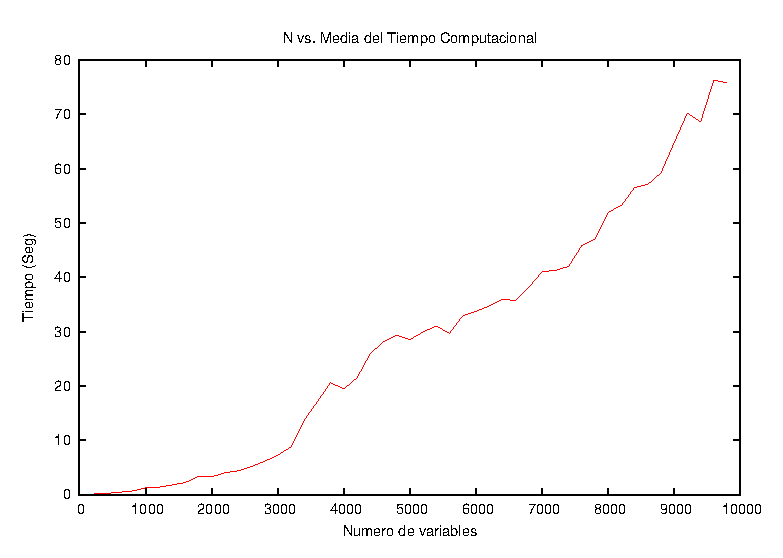
\includegraphics[scale=0.6]{img/Media_Tiempo_1.eps}
%\caption{}
%\end{figure}
%
%\begin{figure}[h]
%\center
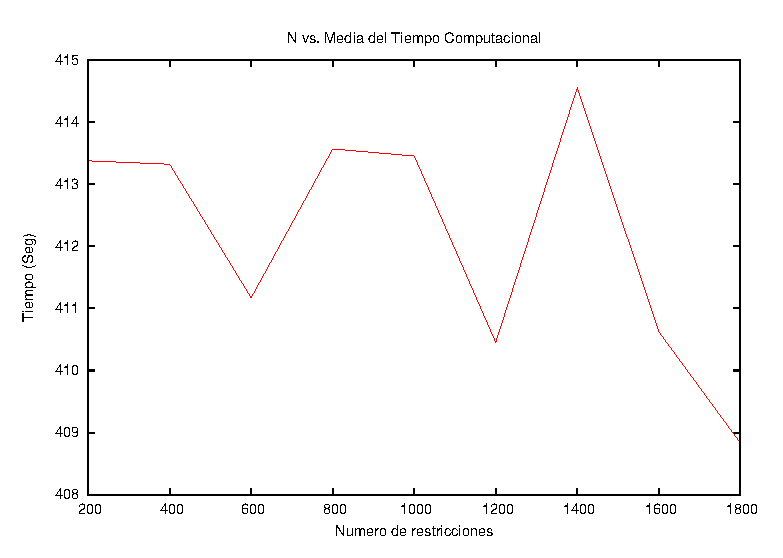
\includegraphics[scale=0.6]{img/Media_Tiempo_2.eps}
\caption{En la izquierda la media contra tiempo con $n=200*i$ e $i \in \{1,2,..,50 \}$ donde $m=n/2$ y en la deracha la media contra tiempo con $n=2000$ donde $m=200*i$.}
\label{img:Media}
\end{figure*}

\begin{figure*}[h]
\center
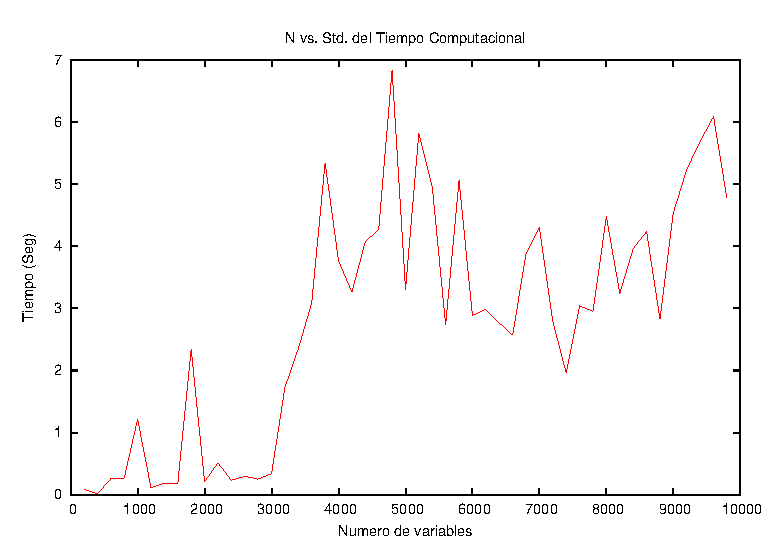
\includegraphics[scale=0.6]{img/Varianza_Tiempo_1.eps}
%\caption{Varianza contra tiempo con $n=200*i$ e $i \in \{1,2,..,50 \}$ donde $m=n/2$.}
%\end{figure}
%
%\begin{figure}[h]
%\center
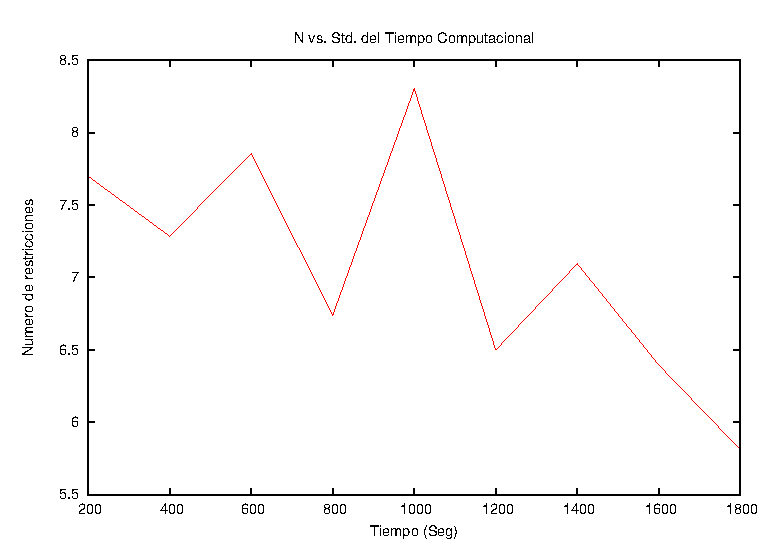
\includegraphics[scale=0.6]{img/Varianza_Tiempo_2.eps}
\caption{En la izquierda la varianza contra tiempo con $n=200*i$ e $i \in \{1,2,..,50 \}$ donde $m=n/2$ y en la derecha la varianza contra tiempo con $n=2000$ donde $m=200*i$.}
\end{figure*}

\subsection{Problema de asignación de ambulancias aéreas}
El objetivo es determinar una signación de costo mínimo de helicoperos a los sitios que satisfacen la demanda proyectada para el siguiente periodo de tiempo.
%
\subsubsection{Declaración del problema}
El servicio de ambulancia tiene un conjunto de ubicaciones con un número de helicópteros en cada sitio.
%
Cada sitio requerido es visitado por su respectivo helicoptero.
%
Existe un costo en la reasignación de un helicóptero a un sitio distinto.
%
Por lo tanto, el servicio proporcionado desea determinar un costo de asignación mínimo de helicópteros a los sitios para satisfacer la demanda en el siguiente periodo de asignación proyectado en cada sitio.
%
\subsection{Formulación matemática}
Dado un conjunto de ubicaciones, las distancias entre las ubicaciones, el número de helicópteros recientemente asignados a cada ubicación, la demanda proyectada para cada ubicación y el costo por ilómetro,
%
El objetivo del problema de asignación de ambulancias es determinar el costo mínimo en la reasignación para satisfacer la demanda proyectada.
%
El problema puede ser formulado como un problema de programación lineal porque la función objetivo y las restricciones son todas funciones lineales.
%
Los pares de distancia son calculadas con la distancia Euclídea.
%


\subsubsection*{Asignar}
\textbf{L} = el conjunto de ubicaciones.


\subsubsection*{Parámetros}
\begin{itemize}
\item \textbf{$x_i$} = la coorenada X para la ubicación de $i, \forall i \in L$.
\item \textbf{$y_i$} = la coorenada Y para la ubicación de $i, \forall i \in L$.
\item \textbf{$d_i$} = demanda proyectada para el sigueinte periodo de la ubicación $i, \forall i \in L$.
\item \textbf{$s_i$} = número de helicópteros recientemente asignados a la ubicación $i, \forall i \in L$.
\item \textbf{$c$} = costo de transportar por kilómetro.
\item \textbf{$dist_{ij}$} = Distancia Euclídea entre la ubicación $i$ y la ubicación $j$ $, \forall i \in L, \forall j \in L$.
\item \textbf{$dist_{ij}$} = $\sqrt{ (x_j - x_i)^2 + (y_j - y_i)^2 }$.
\end{itemize}

\subsubsection*{Variables}
$z_{ij}$ = número de helicópteros a ser desplazados de la ubicación $i$ a la $j$, $\forall i \in L, \forall j \in L$.

\subsubsection*{Función objetivo}
\begin{equation}
Minimizar \quad \sum_{(i,k) \in LxL} dist_{ij} * c * z_{ij}
\end{equation}
\subsubsection*{Restricciones}
Restricciones de balance para cada ubicación $i$ en el conjunto $L$.
\begin{equation}
\sum_{j \in L} z_{ij} + s_i = d_i 6 \sum_{j \in L} z_{ij}, \forall i \in L
\end{equation}

Como ejemplo, se considera un servicio de ambulancias aéreas con 5 ubicaciones en Midwest.
%
La empresa tiene la necesidad de reubicar a los helicópteros basados en le demanda mensual proyectada para cada ubicación.
%
El costo de reasignar un helicóptero del sitio $i$ al sitio $j$ es de $100$ pesos por kilómetro.
%
Se muestra la tabla de cada ubicación.
\begin{table}[]
\centering
\caption{Información de los helicópteros asignados}
\label{my-label}
\begin{tabular}{c|c|c|c|c}
\hline
\textbf{} & \textbf{X - Coord} & \textbf{Y-Coord} & \textbf{\# Assigned} & \textbf{Projected Demand} \\ \hline
Location \#1 & 36 & 20 & 6 & 7 \\ \hline
Location \#2 & 23 & 30 & 2 & 3 \\ \hline
Location \#3 & 23 & 56 & 3 & 2 \\ \hline
Location \#4 & 10 & 15 & 3 & 4 \\ \hline
Location \#5 & 5 & 5 & 4 & 2 \\ \hline
\end{tabular}
\end{table}

La solución al problema es: $z_{3,2}=1$, $z_{5,1}=1$, y $z_{5,4}=1$ con un valor de la función objetivo de $7161.87$.
%
La distancia están como sigue: $dist_{3,2}=26$, $dist_{5,1}=34.438$, y $dist_{5,4}=11.180$.


%
%\section{Resultados}
%\label{Sec:ExperimentalValidation}
%\input{ExperimentalValidation.tex}
%
%\section{Conclusion}
%\label{Sec:Conclusion}
%\input{Conclusion.tex}





% if have a single appendix:
%\appendix[Proof of the Zonklar Equations]
% or
%\appendix  % for no appendix heading
% do not use \section anymore after \appendix, only \section*
% is possibly needed

% use appendices with more than one appendix
% then use \section to start each appendix
% you must declare a \section before using any
% \subsection or using \label (\appendices by itself
% starts a section numbered zero.)
%


%\appendices
%\section{%Proof of the First Zonklar Equation}
%Appendix one text goes here.

% you can choose not to have a title for an appendix
% if you want by leaving the argument blank
%\section{}
%Appendix two text goes here.


% use section* for acknowledgment
%\section*{%Acknowledgment}

%The authors would like to thank...


% Can use something like this to put references on a page
% by themselves when using endfloat and the captionsoff option.
\ifCLASSOPTIONcaptionsoff
  \newpage
\fi



% trigger a \newpage just before the given reference
% number - used to balance the columns on the last page
% adjust value as needed - may need to be readjusted if
% the document is modified later
%\IEEEtriggeratref{8}
% The "triggered" command can be changed if desired:
%\IEEEtriggercmd{\enlargethispage{-5in}}

% references section

% can use a bibliography generated by BibTeX as a .bbl file
% BibTeX documentation can be easily obtained at:
% http://mirror.ctan.org/biblio/bibtex/contrib/doc/
% The IEEEtran BibTeX style support page is at:
% http://www.michaelshell.org/tex/ieeetran/bibtex/
\bibliographystyle{IEEEtran}
% argument is your BibTeX string definitions and bibliography database(s)
\bibliography{bibtex/bib/IEEEabrv,bibtex/bib/References.bib}
%
% <OR> manually copy in the resultant .bbl file
% set second argument of \begin to the number of references
% (used to reserve space for the reference number labels box)
%\begin{thebibliography}{1}

%\bibitem{IEEEhowto:kopka}
%H.~Kopka and P.~W. Daly, \emph{A Guide to \LaTeX}, 3rd~ed.\hskip 1em plus
%  0.5em minus 0.4em\relax Harlow, England: Addison-Wesley, 1999.

%\end{thebibliography}

% biography section
% 
% If you have an EPS/PDF photo (graphicx package needed) extra braces are
% needed around the contents of the optional argument to biography to prevent
% the LaTeX parser from getting confused when it sees the complicated
% \includegraphics command within an optional argument. (You could create
% your own custom macro containing the \includegraphics command to make things
% simpler here.)
%\begin{IEEEbiography}[{\includegraphics[width=1in,height=1.25in,clip,keepaspectratio]{mshell}}]{Michael Shell}
% or if you just want to reserve a space for a photo:


%\begin{IEEEbiography}{Joel Chac\'on}
%Biography text here.
%\end{IEEEbiography}


% if you will not have a photo at all:
%\begin{IEEEbiographynophoto}{John Doe}
%Biography text here.
%\end{IEEEbiographynophoto}

% insert where needed to balance the two columns on the last page with
% biographies
%\newpage

%\begin{IEEEbiographynophoto}{Jane Doe}
%Biography text here.
%\end{IEEEbiographynophoto}

% You can push biographies down or up by placing
% a \vfill before or after them. The appropriate
% use of \vfill depends on what kind of text is
% on the last page and whether or not the columns
% are being equalized.

%\vfill

% Can be used to pull up biographies so that the bottom of the last one
% is flush with the other column.
%\enlargethispage{-5in}



% that's all folks
\end{document}


